\chapter{Methodology}

As stated in the introduction the main goals of this work are:

\begin{itemize}
	\item To design and implement sustainable information systems that can support the long-term preservation of networked crypto art
	\item To contribute to the body of knowledge in the area of networked crypto art conservation
\end{itemize}

From a methodological perspective, the first goal is the one that requires unpacking into actionable and answerable research questions, whereas the second goal will be collaterally achieved from treating the first.

\section{Research Questions}

The first question that must be addressed is one of scope. How many networked OBJKTs are there on the HEN smart contract? Currently this is not known, because there is a single category, \emph{Interactive OBJKTs} for all artworks with mime-type \texttt{application/x-directory}, and there is no information about whether or not they make external network calls. In addition to that, as already established in the introduction, we know that SVG OBJKTs (mime-type \texttt{image/svg+xml}) can also contain embedded scripts and thus can make network calls. So now we have 2 groups of OBJKTs but no idea how to identify the ones of interest to this study. For this reason the first research question is:

\begin{itemize}
	\item RQ1: Can we determine which code-based HEN OBJKTs are networked?
\end{itemize}

Then there is the issue of documenting what these network calls look like in terms of the data structures being transmitted between the OBJKT and their external environmet, so that they can inform conservators when the need arises to perform conservation interventions. At the same time, if we document these network calls, then perhaps we can also examine the rendering of the OBJKT so as to capture its aesthetic evolution. This leads to research question 2:

\begin{itemize}
	\item RQ2: Can we capture and document networked HEN OBJKTs aesthetic evolution?
\end{itemize}

Finally we turn out attention to the sustainability aspect of our goal. There is a wide range of elements involved the sustainability of digital archives \cite{visDigitalArchivingSustainable2024}, however as suggested in the introduction, the low hanging-fruit problem that we want to address first is that of economic sustainability. Even if infrastructure costs of digital archives are normally thwarted by the human resources costs \cite{CostsDigitalRepositories}, the assumption for this study is that, just like Teia, this project will rely on unpaid volunteer work. Therefore, two final research questions can be asked: 

\begin{itemize}
	\item RQ3: What are the disk space requirements for storing all code-based HEN OBJKTs' media assets?
	\item RQ4: Can an online archive for HEN OBJKTs be economically self-sustainable?
\end{itemize}

\vspace{0.5cm}

\begin{table}[h!]
\centering
\footnotesize
\begin{tabular}{|c|p{10cm}|}
\hline
\textbf{RQ\#} & \textbf{Research Question} \\ \hline
RQ1 & Can we determine which code-based HEN OBJKTs are networked? \\ \hline
RQ2 & Can we capture and document networked HEN OBJKTs aesthetic evolution? \\ \hline
RQ3 & What are the disk space requirements for storing all code-based HEN OBJKTs' media assets? \\ \hline
RQ4 & Can an online archive for HEN OBJKTs be economically self-sustainable? \\ \hline
\end{tabular}
\caption{Research Questions}
\end{table}


Based on these questions, the most appropriate methodological choices can be made.

\section{Philosophical Paradigm}

Pragmatism was adopted as the philosophical paradigm for this research. This choice was made based on two factors: the work is highly practical in nature and pragmatism focuses on the practical nature of things and how they bring value and; pragmatism stood out as the best fit for the research methodology which was best aligned with the needs of this work, and which will be discussed in \autoref{sec:methodology}.

Theories are meant to explain a true account of reality, however our view of reality is subjective, so how can we know if a theory is true? \citeauthor{marchDesignNaturalScience1995} note that ``natural science theories receive confirmatory support from the facts that bridges do not collapse, medical treatments cure diseases, people journey to the moon, and nuclear bombs explode'', and propose that ``truth essentially is what works in practice'' \citeyear[p.255]{marchDesignNaturalScience1995}.


\section{Research Approaches}

For the most part this study relies on an inductive approach. For example, when approaching RQ1, the system must automatically detect and classify which OBJKTs are networked. To test the validity of the solution, a sample of OBJKTs which were manually classified is compared with the output of the system, and if all the items are properly classified then we can generalise that the automatic classification works for all cases.
A similar approach is applied to the other research questions.


\section{Research Methodology}
\label{sec:methodology}

This study will follow a Design Science Research (\indexacronym{dsr}) methodology, which is a well established methodology in the field of IS, and one where
"knowledge and understanding of a problem domain and its solution are achieved in the building and application of the designed artefact"  \cite[p.75]{hevnerDesignScienceInformation2004}.

Hevner et al \citeyear{hevnerDesignScienceInformation2004} describe DSR as having a dual set of core values: relevance and rigor. On the relevance side, the business, or in our case the community, reveals the need for the artifact by expressing a set of needs. Whereas on the rigor side, the design and development of the artifact is informed by applicable knowledge from theories, frameworks and other elements of the knowledge base. See \autoref{fig:is-research-framework}.

In the context of the artifact being developed, three main roles of stakeholders are identified: artists, collectors and conservators.

\begin{figure}[h]
    \centering
    \includesvg[width=\textwidth]{is-research-framework}
    \caption[Information Systems Research Framework]{Information Systems Research Framework. Source: \cite[p.80]{hevnerDesignScienceInformation2004}}
    \label{fig:is-research-framework}
\end{figure}


\section{Research Methods}

This study primarily follows a quantitative research method, namely the systematic collection and analysis of the data produced by the artifact, in order to validate the artifact's ability to classify and document the OBJKTs as well as to determine the infrastructure requirements and financial costs.

In a secondary role, a qualitative strategy was also employed, with stakeholder interviews, to gather additional evidence of the accuracy of the artifact in classifying networked OBJKTs, and to receive feedback which may be useful for future iterations of the artifact.

Even though both methodologies are used, due to the lack of integration or triangulation between them, this study cannot be classified as having a mixed methodology \cite{turnerResearchDesignMixed2017}.


\subsection{Research Question Driven Development}

In order to address the research questions, a new iterative development method was conceived, inspired in the agile development method \cite{shoreArtAgileDevelopment2021} but simplified and focused on answering the research questions. We'll call this method Research Question Driven Development (\indexacronym{rqdd}).

This process involves the development of an information system, the main artifact, and the observation of that artifact in a real world scenario. Each iteration is designed to either answer a research question, or to bring the artifact closer to such an answer in developmental terms.

The iterative development method is illustrated in \autoref{fig:research-method-plan}.

\begin{figure}[h]
    \centering
    \includesvg[width=0.75\textwidth]{research-method-plan}
    \caption[Research Question Driven Development]{Research Question Driven Development}
    \label{fig:research-method-plan}
\end{figure}

For each research question the following steps were taken:

\begin{enumerate}
    \item \textbf{Design}: a design of the system components required to address the question was formulated. Following the pragmatic philosophy and with a rapid speed of development cycles, this step was often a mental process, rather than formalised as a diagram;
    \item  \textbf{Build}: the design was implemented through coding
    \item  \textbf{Run}: the implemented components were ran against real world data
    \item  \textbf{Observe}: the behaviour of the system was observed
\end{enumerate}

After each iteration, if the observation satisfied the research question, the design was formalised as a model so as to contribute to the knowledge base, a new research question was selected, and the iterative process would continue. If, on the other hand, the observation did not satisfy the research question, then the process would restart, either with a refining of the same design or with a new design approach.

A key aspect of this approach is that it is the research questions that drive the development plan, rather than a set of initial requirements gathered by the stakeholders. This is intentional and does not dismiss the needs of the stakeholders. Much the opposite. By focusing on the research questions and bringing the artifact closer to solving the main goals, this method will contribute back to the environment or context of the stakeholders at faster rate than if the development effort were to deal with a much wider and fragmented set of requirements. Once the artifact reaches a state where it can perform its core functions, then the methodology can incorporate evaluations and feedback by stakeholders who, after experiencing the artifact in action, will have a clearer understanding of its intended functions and will be in a position to provide more valuable feedback.

Another key benefit of \gls{researchquestiondrivendev} is that, in the context of an DSR research methodology, the answering of the research questions constitutes the evaluation and validation of the artifact.

Finally, this method aligns with the Pragmatism paradigm, which serves as the theoretical foundation of this study.

\subsection{Descriptive Statistics}

In order to answer the research questions, the data generated by the artifact was exported from the artifact's database in tabular form, by means of a CVS file, and imported into the R statistics program, where it was analysed with the use of descriptive statistics.

\subsection{Interviews with Stakeholders}

Even though not directly related to the research questions, semi-structured interviews were undertaken with stakeholders in order to provide a formative evaluation of the artifact, with the goal of refining and improving it in the future. The findings from these interviews will inform future work on the artifact.

\todo
A total of 3 stakeholders were interviewed, through voice calls on Discord and a Google Meet videocall: 2 artists and a conservator.


\section{Reproducibility}

In order to facilitate the reproducibility of the findings, all the source code and data collected (except interviews) was made available publicly:

\begin{enumerate}
    \item the source code of the artifact is available at:\\ \texttt{https://github.com/seda-studio/arkivo}
    \item the data exported from the database, and the R source files are available at: \todo
\end{enumerate}


\todo development environment

\todo tools used


\section{Research and Development Tools}


\subsection{Journaling}

During the research and development, journaling was employed as a research method, primarily using two tools:

\begin{enumerate}
    \item Obsidian\footnotemark[1]: a note taking desktop app, for text-based note taking. This app allows rich formatting of notes using Markdown, and the linking of documents together, similarly to a wiki. It was useful to be able to quickly copy/paste text excerpts, quotes, code snippets, and other bits of information which were useful to record for later use;
    \item Goodnotes\footnotemark[2]: a note taking mobile app, for hand-written notes on a tablet device like an iPad. This was used as the primary idea brainstorming tool, but also to take notes whenever the work laptop was not readily available. It syncs with a companion desktop app, so the notes would also be available on the work laptop.
\end{enumerate}

Below are samples of notes taken with these tools:


\begin{figure}[H]
  \centering
  \begin{subfigure}[b]{0.45\textwidth}
    \centering
    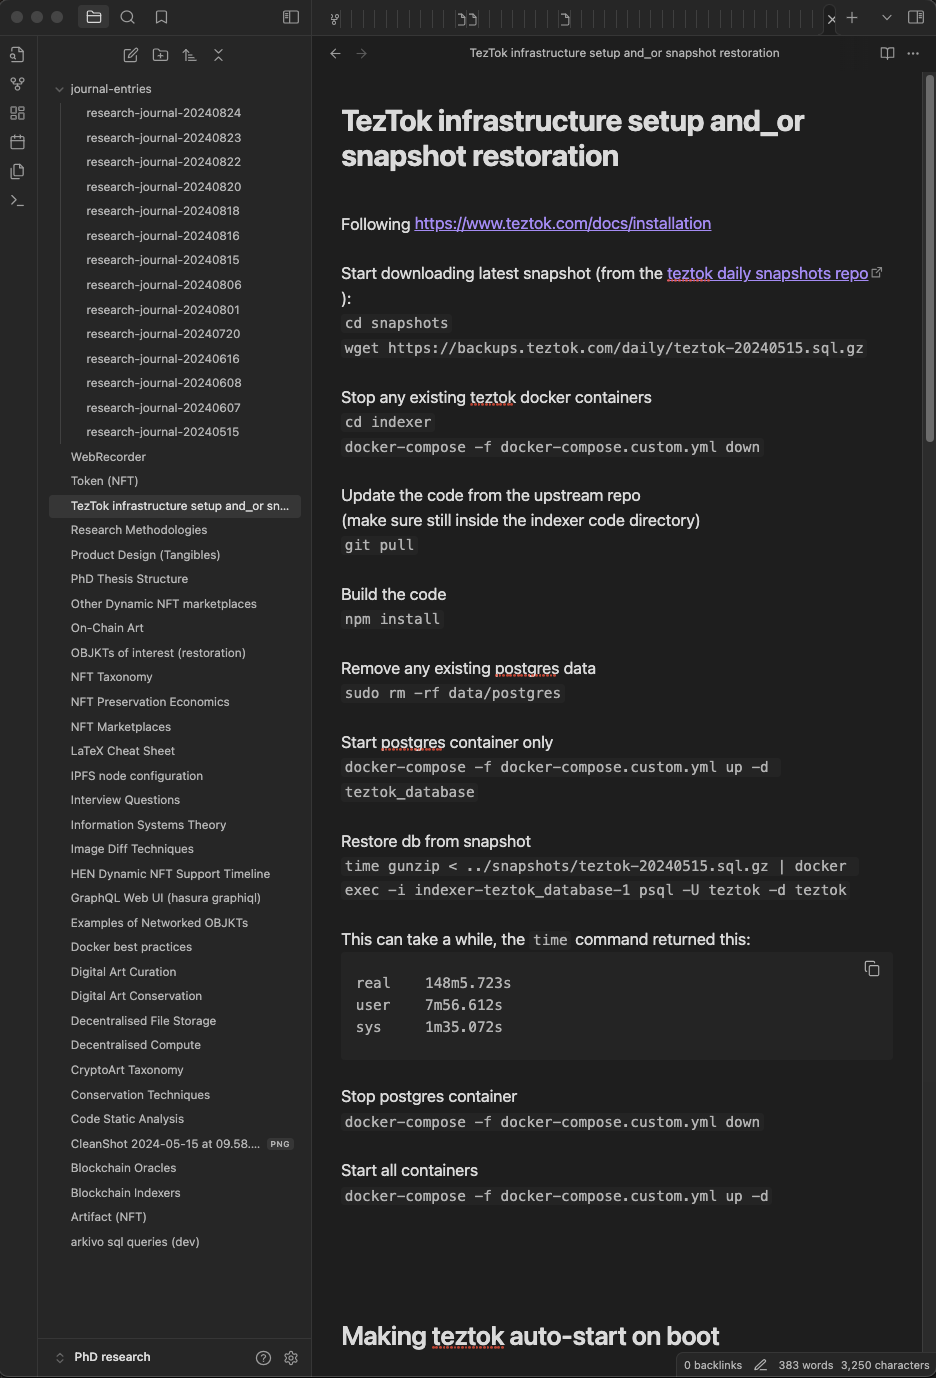
\includegraphics[width=0.75\textwidth]{obsidian.png}
    \caption[Sample Journal Entry in Obsidian]{Sample Journal Entry on Obsidian}
    \label{fig:obsidian}
  \end{subfigure}
  \hfill
  \begin{subfigure}[b]{0.45\textwidth}
    \centering
    \begingroup
    \setlength{\fboxsep}{0pt} % No padding between box and content
    \setlength{\fboxrule}{0.5pt} % Thickness of the border
    \fcolorbox{gray}{white}{\includegraphics[width=0.75\textwidth, page=1]{handwritten-notes.pdf}}
    \endgroup
    \caption[Sample Journal Entry in GoodNotes]{Sample Journal Entry in GoodNotes}
    \label{fig:goodnotes}
  \end{subfigure}
  \caption{Sample Journal Entries}
  \label{fig:sample-journal}
\end{figure}




\footnotetext[1]{https://obsidian.md/}
\footnotetext[2]{https://www.goodnotes.com/}


\subsection{Thesis Writing}

This thesis was written using LaTeX, a free and open source software system for typesetting documents, which is widely popular in the communication and publication of scientific documents. The main reason for this choice was a concern that Microsoft Word might struggle in terms of performance when dealing with an increasingly large document, with many images, and references. From this point of view this proved to be a wise decision, as the full thesis can be rendered to a PDF file in less than 10 seconds. However it also proved to be a double-edged sword. LaTeX is a complex system, with many commands and configuration options, some of which may have unexpected interactions with each other. Several times unexpected formatting errors occurred in one part of the document, whilst attempting to fix another part, because of these interactions.
It needs to be noted that when dealing with these problems, ChatGPT was an invaluable tool. Most of the technical issues were resolved simply by copy/pasting the LaTeX document source code into a prompt and describing the issue that was happening in the rendered document. Invariably the LLM would identify the issue and suggest the correct LaTeX commands to solve it. If ChatGPT were a person, it would have featured in the acknowledgments section of this thesis.

The editing was done in TeXShop, a free and open source visual editor for MacOS, and the document was structured as one main file, which contained the preamble and overall document structure, and then individual chapters were included as separate files. Frontmatter sections, such as the title, abstract, and acknowledgments, were also all separated into individual files. This allowed for easier browsing and scrolling of each section, however when searching for text across the whole document one must then rely on the rendered PDF.



For most diagrams Google Draw, which is a part of the Google Docs suite, was used. The reason for this is that it allowed for very fast diagram sketching, which can be exported as \indexacronym{svg} files. Then these files can be imported into the LaTeX document and adjusted for size without any loss of quality.

Inkscape, another free and open source vector graphics tool, was used to extract vector-based diagrams from existing literature. For example, \autoref{fig:is-research-framework} in page \pageref{fig:is-research-framework}, is a vector based diagram which was exported from the original article PDF, using Inkscape. Care was taken to convert all text into vector paths, so as to scale properly in this document.


